Since all used UHV chambers have many common part, a typical setup is described with the LT-STM setup. Here the most experiments were carried out.

\paragraph{Vacuum system}
\paragraph{Cooling system} 
While low temperature (LT) STMs may be operated with solely helium, it is more resource-saving to cool the direct proximity of the sample and the STM with He, but to suppress the heat flow out of the He-cryostat with a second surrounding nitrogen cryostat (boiling point: \SI{77}{\K}, compare figure \ref{fig:STM-cryo}). This diminishes consumption of globally limited and rather expensive He. To maintain a temperature of \SIrange{5}{7}{\K}, one to two liters of liquid helium are required a day, plus an additional amount of three to four liters liquid nitrogen. Evaporated helium is reclaimed in a closed circuit with a system of purifying and storage/cooling steps so that only a small amount of helium escapes the circuit and is lost.

Sample temperatures down to \SIrange{5}{7}{\K} allow for observations not possible at elevated (room) temperature. Cooling not only reduces thermal drift in the piezo elements that are used to control the tip's position on the sample. Thermal energy at low temperature is not high enough for atoms or molecules to move on most substrates. Species mobile at room temperature (and therefor not representable at room temperature in the sub-ML regime) become immobile and accessible for ST microscopy and spectroscopy. STS spectra resolution is better at low temperatures as discussed in \ref{section:AFM-resolution}.

\begin{figure}[ht]\centering
		\subfigure[LT-STM setup mainly used in this work. Different functional groups are colored in different colors. A low base pressure in achieved with a combined pumping system comprised of ion pumps and turbo molecular pumps (cyan). The liquid helium/nitrogen bath cryostat (red) is used to maintain low temperatures. Sample holders are operated with a rote able, variable temperature manipulator. Sample preparation is done in a chamber (blue). After transfer to the LT-STM chamber (yellow) a gate valve is used to seal the LT-STM from remaining residual gas that may be present in the preparation chamber. Vibration isolation of the frame is achieved with legs floating on pressurized cylinders.]{
			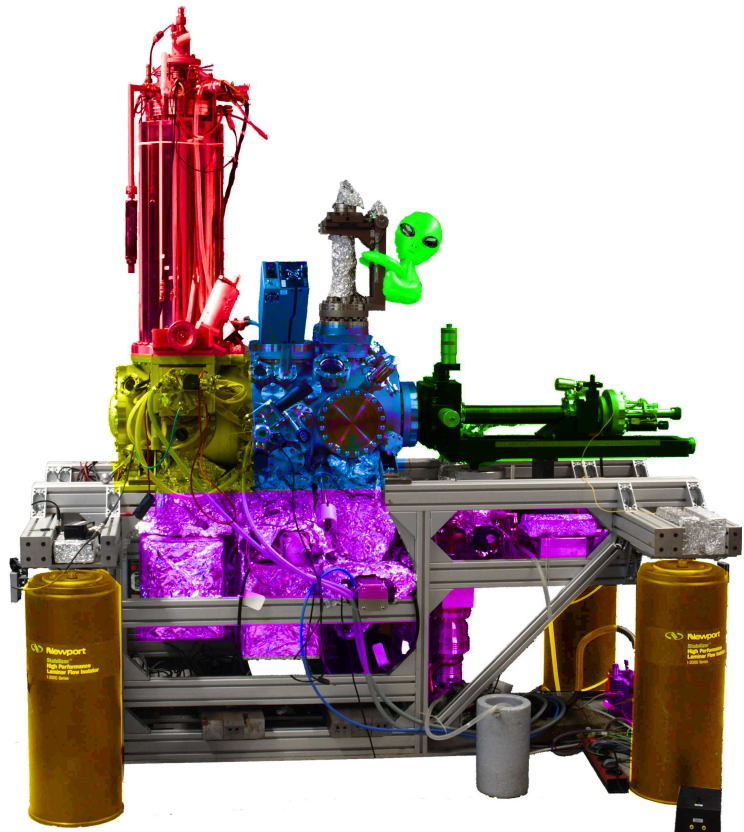
\includegraphics[width=0.45\textwidth]{./images/chamber-sketch.jpg}
			\label{fig:chamber-sketch}
		} \quad
		\subfigure[Scheme of a STM liquid bath cryostat. While in the inner measurement stage a temperature of $\approx \SIrange{5}{7}{\K}$ is achieved with a liquid helium reservoir, an outer liquid nitrogen cryostat is used to isolate the evacuated inner cryostat from the surrounding room temperature.]{
			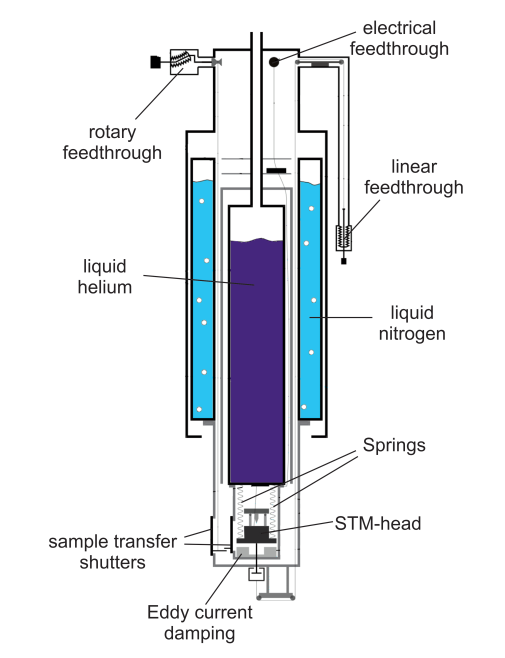
\includegraphics[width=0.45\textwidth]{./images/sketch-cryo.jpg}
			\label{fig:STM-cryo}
		}
	\caption{Typical setup for low temperature measurements. A vibration isolated UHV chamber is used to prepare samples and investigate them in a separable chamber with either STM or AFM. A liquid bath cryostat is used to maintain low temperatures. Images stem from {diss-knud}}
	\label{fig:STM}
\end{figure}

\paragraph{Damping stages}
Two damping stages are used, one for the chamber and a separate one for the STM.
\begin{itemize}
	\item The whole UHV system is placed on air pressurized legs. These can be elevated on demand, so that the chamber floats on four dampers and external vibrations/shocks are damped.
	\item A second stage decouples the sensitive STM from the rest of the setup. First the complete STM stage hangs on springs to further limit the direct influence of vibrations. Second the remaining oscillation amplitude is damped by a eddy current damping. It is made of three magnets in close proximity to the surrounding support so that eddy currents are induced for each minute movement. The eddy current is typically larger at cryogenic temperatures, that results in a damping that works best at low temperatures. The kinetic energy of the oscillating system is transferred by the eddy currents into heat within the surrounding conductor. The heat is then mitigated by the external cooling of the cryostat.
\end{itemize}